\documentclass{SBCbookchapter}
\usepackage[utf8]{inputenc}
\usepackage[T1]{fontenc}
\usepackage[english,brazilian]{babel}
\usepackage{hyperref}
\hypersetup{colorlinks=true,allcolors=black}
\usepackage{graphicx}
\usepackage{picins}

\begin{document}
\section*{Biografia Resumida dos Autores}

~\\

\parpic(3cm,2.5cm)[r][b]{%
  % 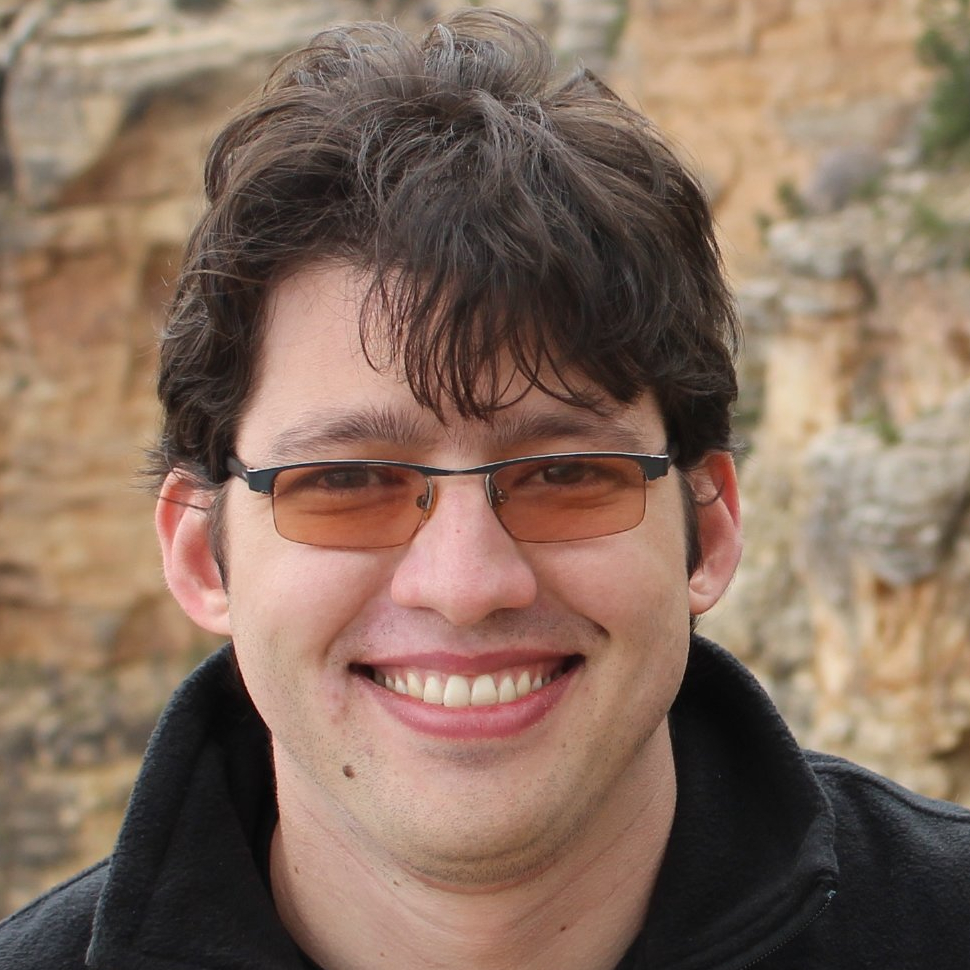
\includegraphics[width=3cm,height=3cm]{photos/roberto}
}
\noindent\textbf{Guilherme F.~Lima} é pesquisador associado do Laboratório
TeleMídia da PUC-Rio.  Seus interesses de pesquisa incluem linguagens de
programação e modelos para sincronismo multimídia.  Obteve o Doutorado em
Informática pela PUC-Rio em 2015.  Também possui Mestrado em Informática (2011)
e Bacharelado em Sistemas de Informação (2009), ambos pela PUC-Rio.
\vspace{1cm}

\parpic(3cm,2.3cm)[r][b]{%
  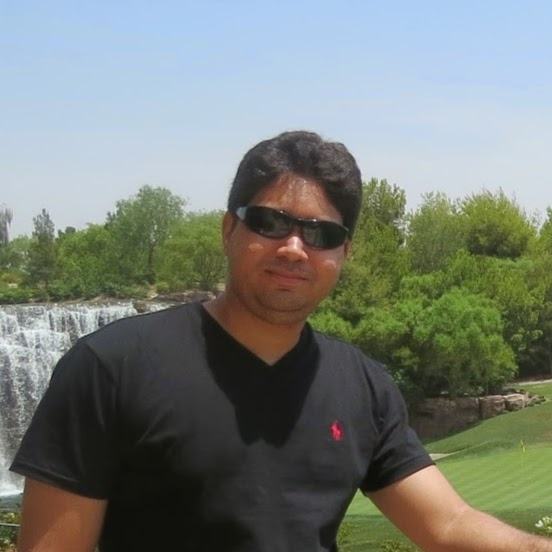
\includegraphics[width=3cm,height=3cm]{photos/rodrigo}
}
\noindent\textbf{Rodrigo C.\,M.~Santos} é doutorando em Informática na PUC-Rio.
Mestre em Ciência da Computação pela Universidade Federal do Maranhão (2013).
Atualmente é pesquisador do laboratório TeleMídia da PUC-Rio e colaborador do
laboratório LAWS/UFMA, tendo como principais interesse de pesquisa: sistemas
multimídia distribuídos, sincronização de mídia em diferentes dispositivos e
linguagens reativas síncronas. 
\vspace{1cm}

\parpic(3cm,2.5cm)[r][b]{%
  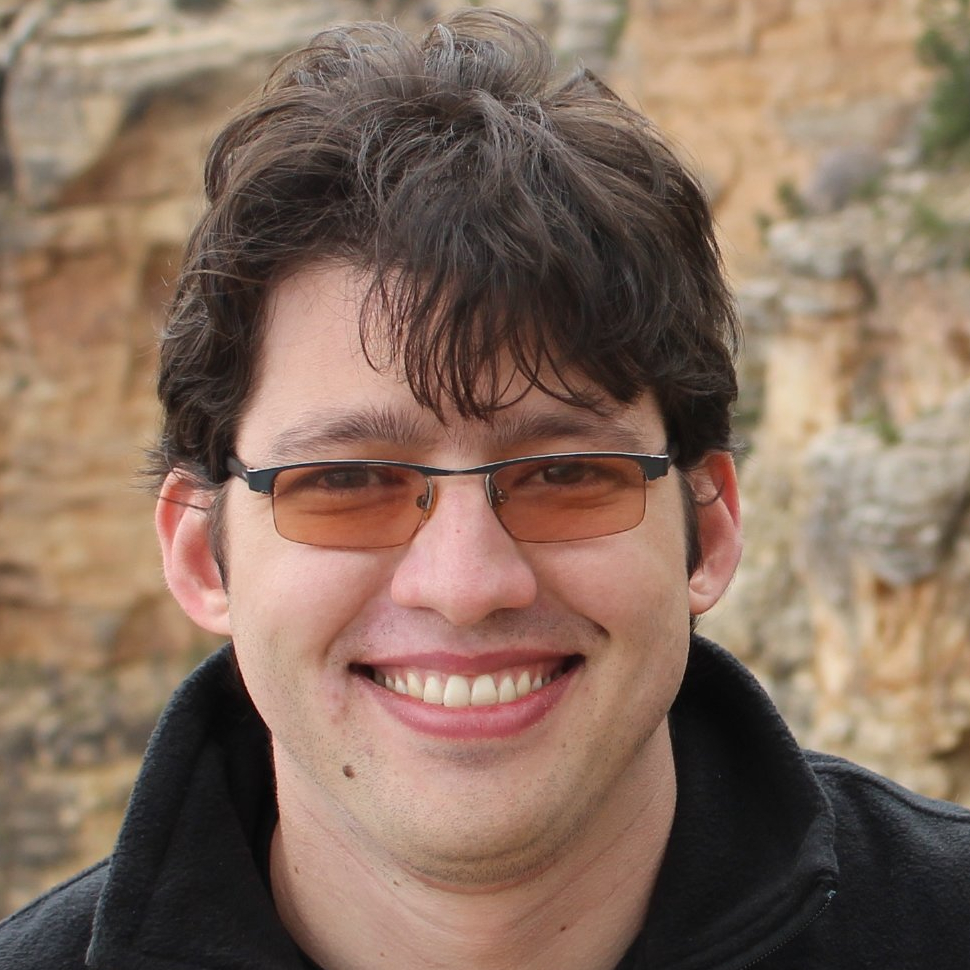
\includegraphics[width=3cm,height=3cm]{photos/roberto}
}
\noindent\textbf{Roberto G.\, de A.~Azevedo} é pesquisador associado do
Laboratório TeleMídia da PUC-Rio. Possui doutorado (2015) e mestrado (2010) em
Informática pela PUC-Rio e é Bacharel em Ciência da Computação pela
Universidade Federal do Maranhão (2008). Seus interesses de pesquisa incluem:
representação e autoria de cenas multimídia interativas; e representação,
codificação, transmissão e renderização de vídeos 3D.

\end{document}

